\begin{Czech}
\section{Software}
\end{Czech}

\begin{Czech}
Systém je přístupný na IP adrese \url{http://192.168.11.196:8123}. Stačí jakýkoliv aktuální webový prohlížeč. Je možné využít i mobilní aplikaci na Android, stažení přímo v Play Store.
\end{Czech}

% ====================  START Tab overview ====================
\begin{Czech}
\subsection{Záložka přehled}
\end{Czech}

\begin{Czech}
V záložce \textbf{přehled} obrázek \ref{fig:tab-overview} (horní modré menu) jsou vidět v jednom grafu v části „Porovnání teploty“ všechny měřené teploty (krby, zásobník otopné vody a venkovní teplota). V části „\textit{Jednotlivé senzory}“ jsou jednotlivé teplotní senzory s aktuálně naměřenou teplotou. 
\end{Czech}

\begin{Czech}
\begin{figure}[H]
    \centering
    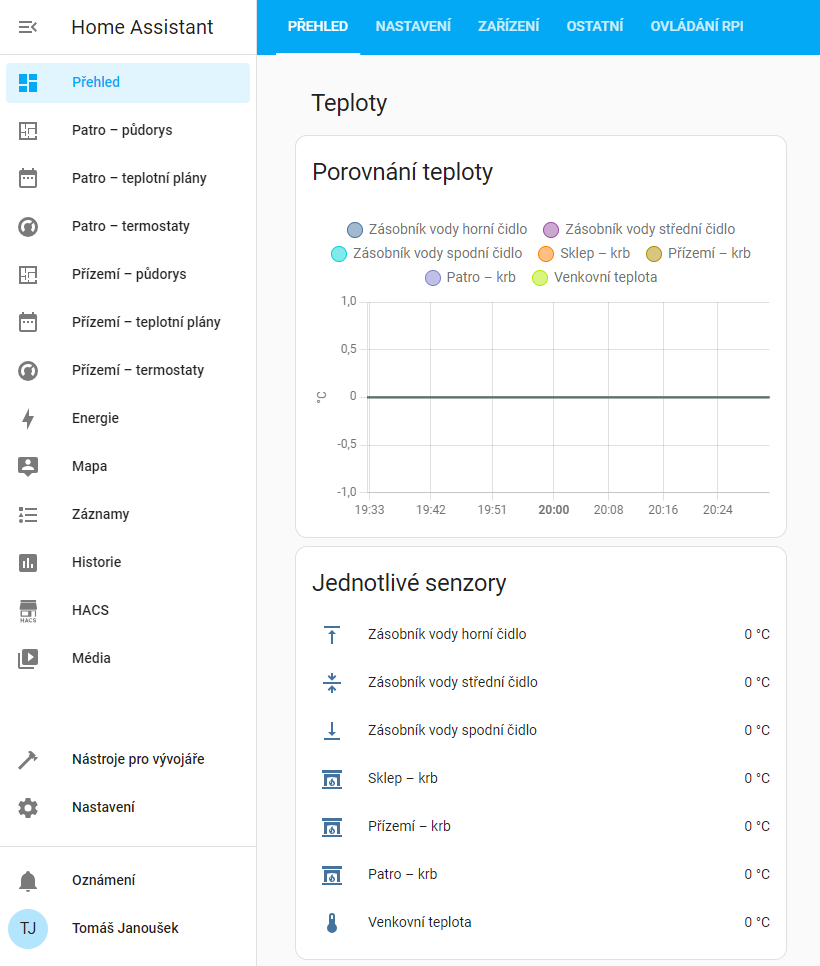
\includegraphics[width=0.9\textwidth]{pictures/czech/software/tab-overview.png}
    \caption{Záložka přehled.}
    \label{fig:tab-overview}
\end{figure}
\end{Czech}

\begin{Czech}
Pokud uživatel klikne na název teplotního senzoru např. Zásobník vody horní, zobrazí se historie naměřených hodnot, obrázek \ref{fig:click-temperature-sensor}. Dvojitým kliknutí na horní část tohoto okna se zobrazené okno ještě zvětší.
\end{Czech}

\begin{Czech}
\begin{figure}[H]
    \centering
    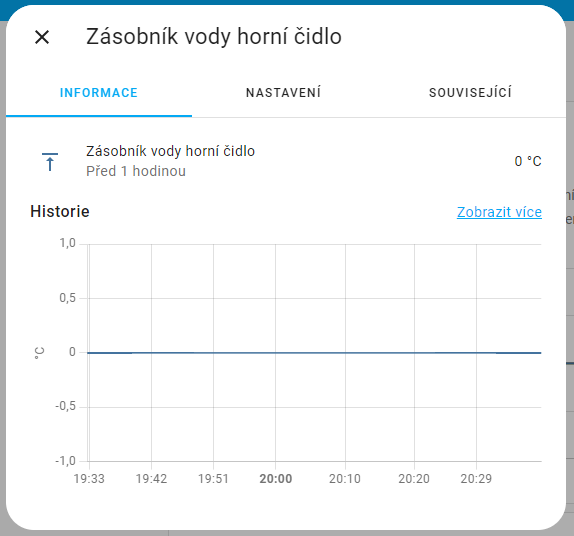
\includegraphics[width=0.6\textwidth]{pictures/czech/software/click-temperature-sensor.png}
    \caption{Zobrazení historie senzoru teplotu po kliknutí na název.}
    \label{fig:click-temperature-sensor}
\end{figure}
\end{Czech}
% ====================  STOP Tab overview ====================

% ====================  START Tab settings ====================
\begin{Czech}
\subsection{Záložka nastavení}
\end{Czech}

\begin{Czech}
V záložce \textbf{nastavení} obrázek \ref{fig:tab-settings} (horní modré menu) jsou vidět módy „\textit{Řízení teploty}“, „\textit{Módy řízení}“, „\textit{Spínání topné spirály}“, „\textit{Krby – spínání čerpadel}“, „\textit{LED indikace – mezní parametry zásobníku teplé vody}“ a „\textit{Ostatní nastavení}“. Jednotlivé možnosti jsou popsány níže.
\end{Czech}

\begin{Czech}
\begin{figure}[H]
    \centering
    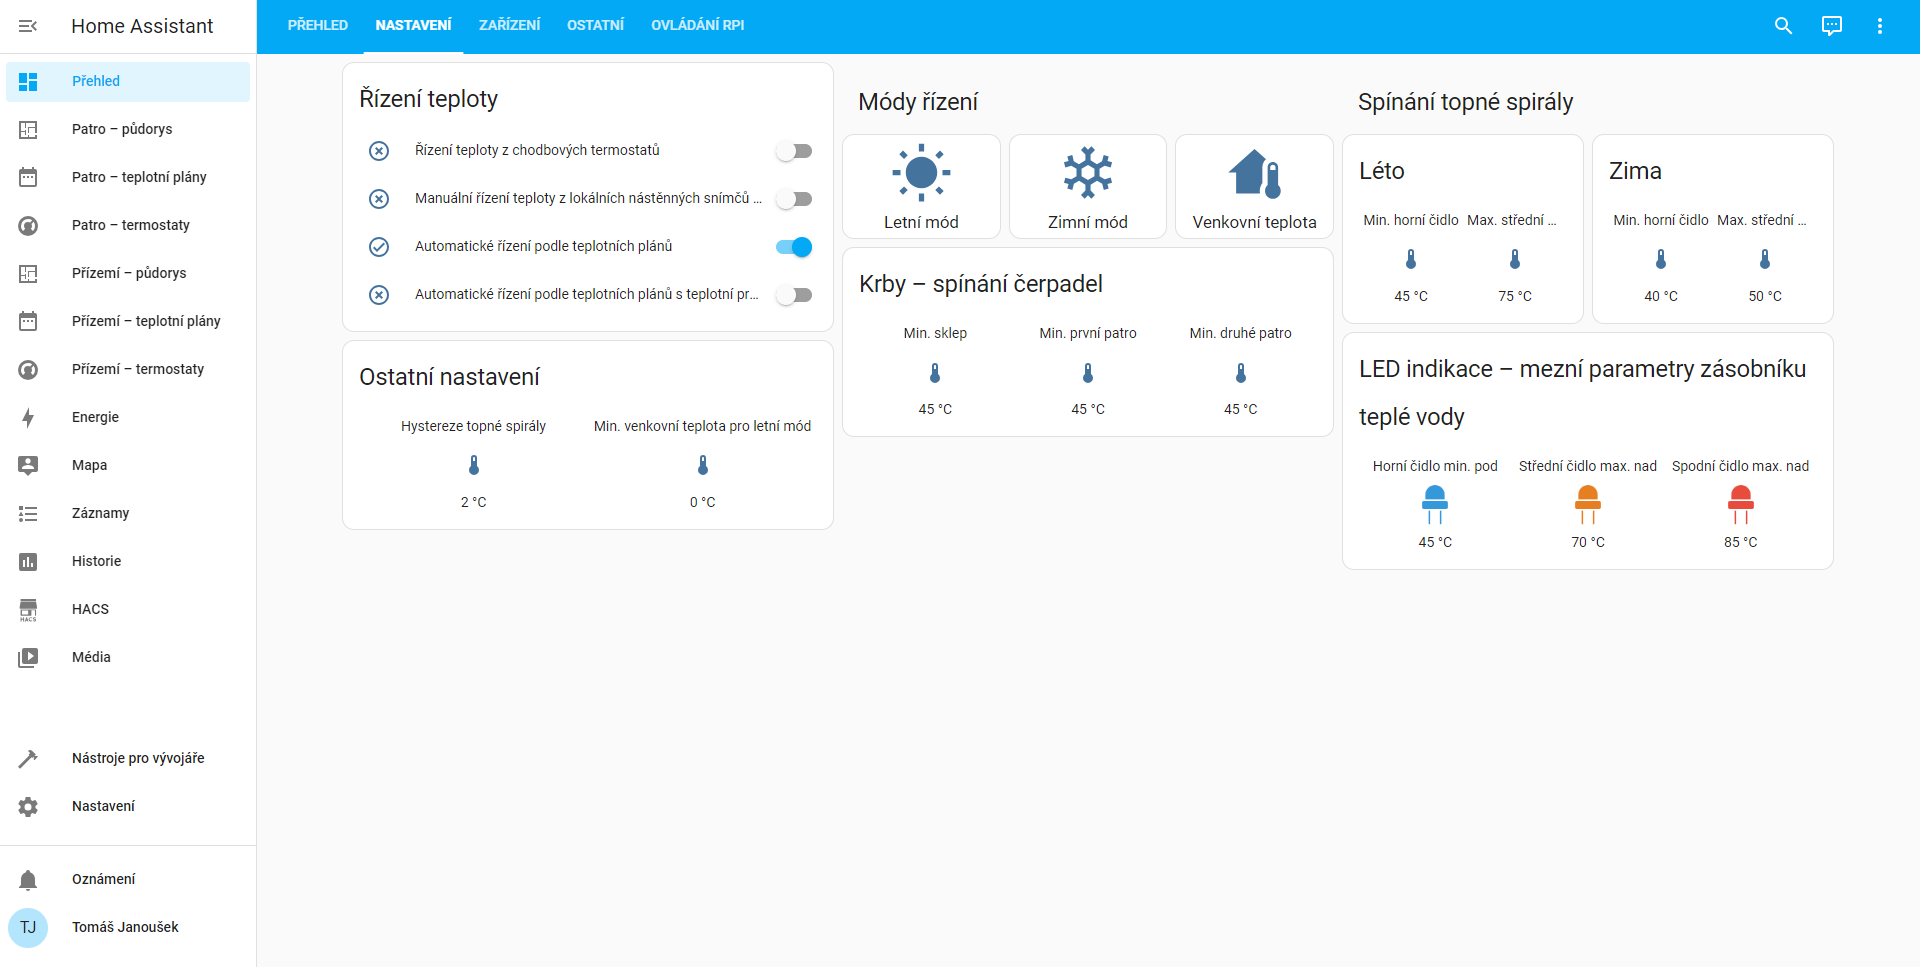
\includegraphics[width=1\textwidth]{pictures/czech/software/tab-settings.png}
    \caption{Záložka nastavení.}
    \label{fig:tab-settings}
\end{figure}
\end{Czech}

% ========================================

\begin{Czech}
\subsubsection{Řízení teploty}
\end{Czech}
\label{sec:temperature-control}

\begin{Czech}
V části nastavení „\textit{Řízení teploty}“ (obrázek \ref{fig:temperature-control}) je možné vybrat z  několika módů. Pro řízení vytápění je nutné vždy vybrat jeden z módů řízení v opačném případě nebude docházet k řízení vytápění podle automatizace.
\end{Czech}

\begin{Czech}
\begin{figure}[H]
    \centering
    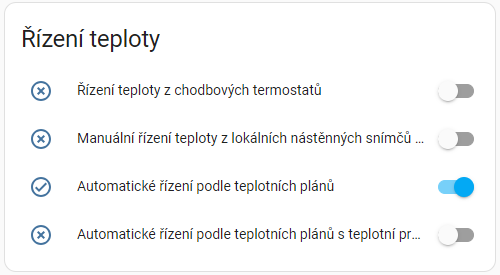
\includegraphics[width=0.6\textwidth]{pictures/czech/software/temperature-control.png}
    \caption{Řízení teploty.}
    \label{fig:temperature-control}
\end{figure}
\end{Czech}

% ========================================

\begin{Czech}
\subsubsubsection{Řízení teploty z chodbových termostatů}
\end{Czech}

\begin{Czech}
V módu „\textit{Řízení teploty z chodbových termostatů}“ docházení na základě nastavené teploty v chodbových termostatech, které jsou umístěné v přízemí a v patře k ovládání všech otopných okruhů pro dané patro. Pokud je požadavek na vytápění, dojde k zapnutí všechny otopných okruhů, jinak dojde k vypnutí. Stav zapnutí jednotlivých chodbových termostatů (stav vytápění) je signalizovány svítící červenou LED přímo na termostatu, případně v systému v \textbf{záložce zařízení} \mbox{v části} „\textit{Termostaty chodby – požadavek topení}“ pro každé patro, obrázek \ref{fig:corridor-thermostats}. Stav jednotlivých otopných okruhů je vidět na \textbf{záložce zařízení} v části „\textit{Přízení nebo patro – otopné okruhy (ventily)}“, obrázek \ref{fig:heating-circuits-ground-floor}.
\end{Czech}

\begin{Czech}
\begin{figure}[H]
    \centering
    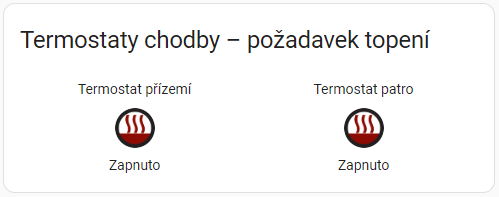
\includegraphics[width=0.6\textwidth]{pictures/czech/software/corridor-thermostats.png}
    \caption{Termostaty chodby – požadavek topení.}
    \label{fig:corridor-thermostats}
\end{figure}
\end{Czech}

\begin{Czech}
\begin{figure}[H]
    \centering
    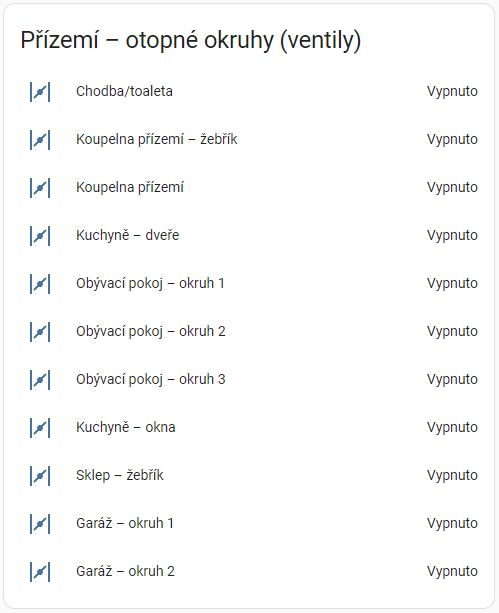
\includegraphics[width=0.6\textwidth]{pictures/czech/software/heating-circuits-ground-floor.png}
    \caption{Přízemí – otopné okruhy (ventily).}
    \label{fig:heating-circuits-ground-floor}
\end{figure}
\end{Czech}

\begin{Czech}
\tipbox{Pozor!}{Toto řízení je funkční jen v případě povolení „Zimní mód“ v části „Módy řízení“. Další popis v části \ref{sec:control-modes} „Módy řízení“.}
\end{Czech}

% ========================================

\begin{Czech}
\subsubsubsection{Manuální řízení teploty z lokálních snímáčů teploty}
\end{Czech}

\begin{Czech}
V módu „\textit{Manuální řízení teploty z lokálních snímáčů teploty}“ dochází k řízení teploty podle daného nástěnného snímače teploty umístěný v každé místnosti. Pro danou místnost jsou následně ovládány otopné okruhy. Stav jednotlivých termostatů je vidět v levém menu v „\textit{Přízemí – termostaty}“ nebo v „\textit{Patro – termostaty}“, obrázek \ref{fig:thermostats-first-floor}. Na každém termostatu (obrázek \ref{fig:thermostat}) lze nastavit požadovanou teplotu pomocí oranžového posuvníku, případně lze kliknout na 3 tečky v pravém horním rohu termostatu a požadovanou teplotu lze nastavit pomocí šipek, obrázek \ref{fig:click-thermostat}. Aktuálně naměřená teplota se zobrazuje uprostřed. Pod každým termostatem je dále informace „\textit{Stav připojení}“, která signalizuje, zda daný snímač je připojen do systému a „\textit{Detekce otevřeného okna}“, která signalizuje, zda došlo k otevření okna v místnosti, v takovém případě dojde k pozastavení vytápění pro danou místnost než se okno opět zavře.
\end{Czech}

\begin{Czech}
\begin{figure}[H]
    \centering
    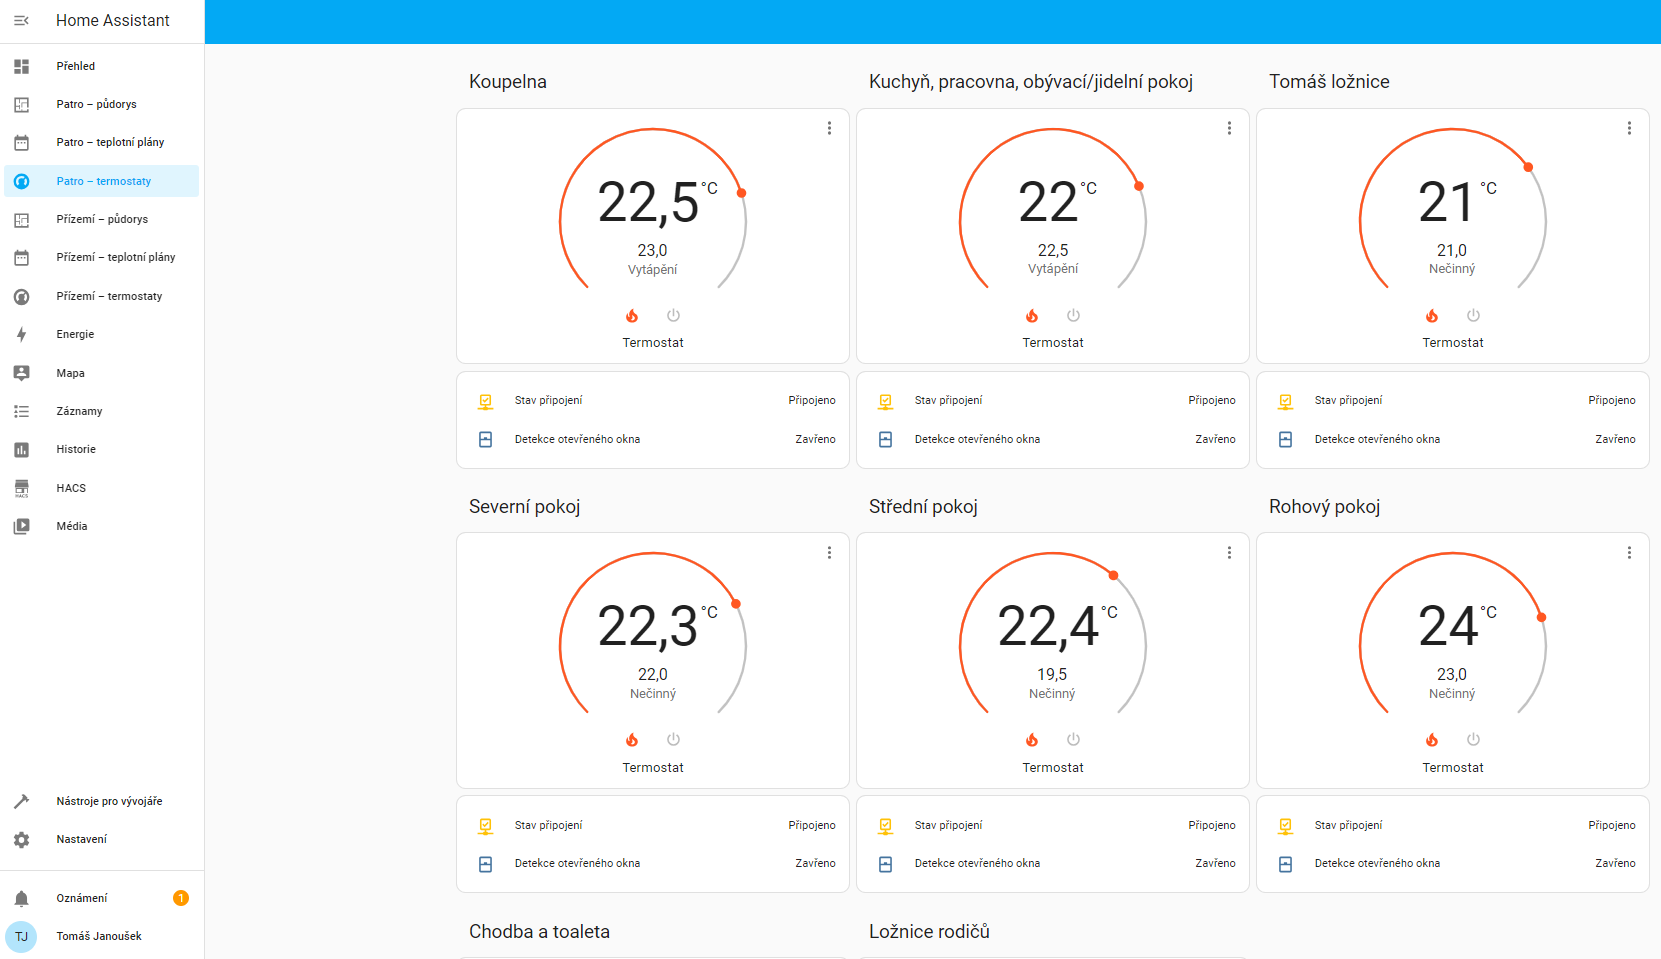
\includegraphics[width=1\textwidth]{pictures/czech/software/thermostats-first-floor.png}
    \caption{Patro – termostaty.}
    \label{fig:thermostats-first-floor}
\end{figure}
\end{Czech}

\begin{Czech}
\begin{figure}[H]
    \centering
    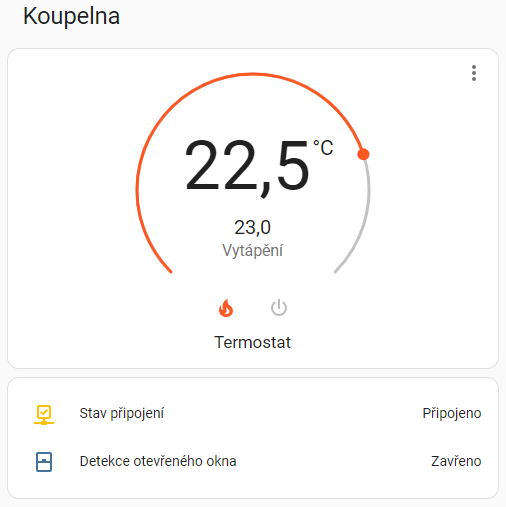
\includegraphics[width=0.5\textwidth]{pictures/czech/software/thermostat.png}
    \caption{Termostat – koupelna.}
    \label{fig:thermostat}
\end{figure}
\end{Czech}

\begin{Czech}
\begin{figure}[H]
    \centering
    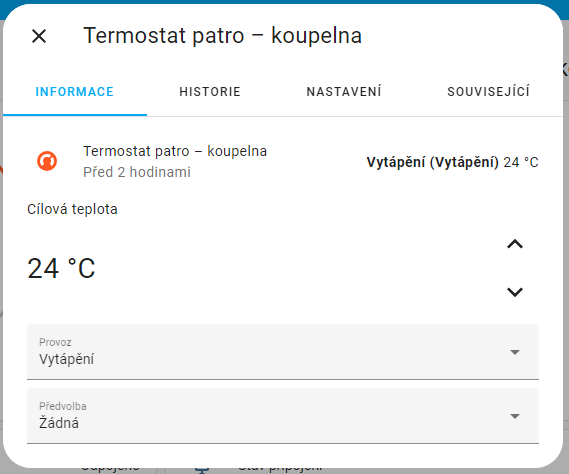
\includegraphics[width=0.5\textwidth]{pictures/czech/software/click-thermostat.png}
    \caption{Kliknutí na 3 tečky v pravém horním rohu termostatu – koupelna.}
    \label{fig:click-thermostat}
\end{figure}
\end{Czech}

% ========================================

\begin{Czech}
\subsubsubsection{Automatické řízení podle teplotních plánů}
\end{Czech}

\begin{Czech}
V módu „\textit{Automatické řízení podle teplotních plánů}“ docházení k řízení vytápění podle nástěnných snímačů teploty pro každou místnost. Dochází však na základě teplotních plánů nastavování požadované teploty, obrázek \ref{fig:temperature-plan-ground-floor}.
\end{Czech}

\begin{Czech}
\begin{figure}[H]
    \centering
    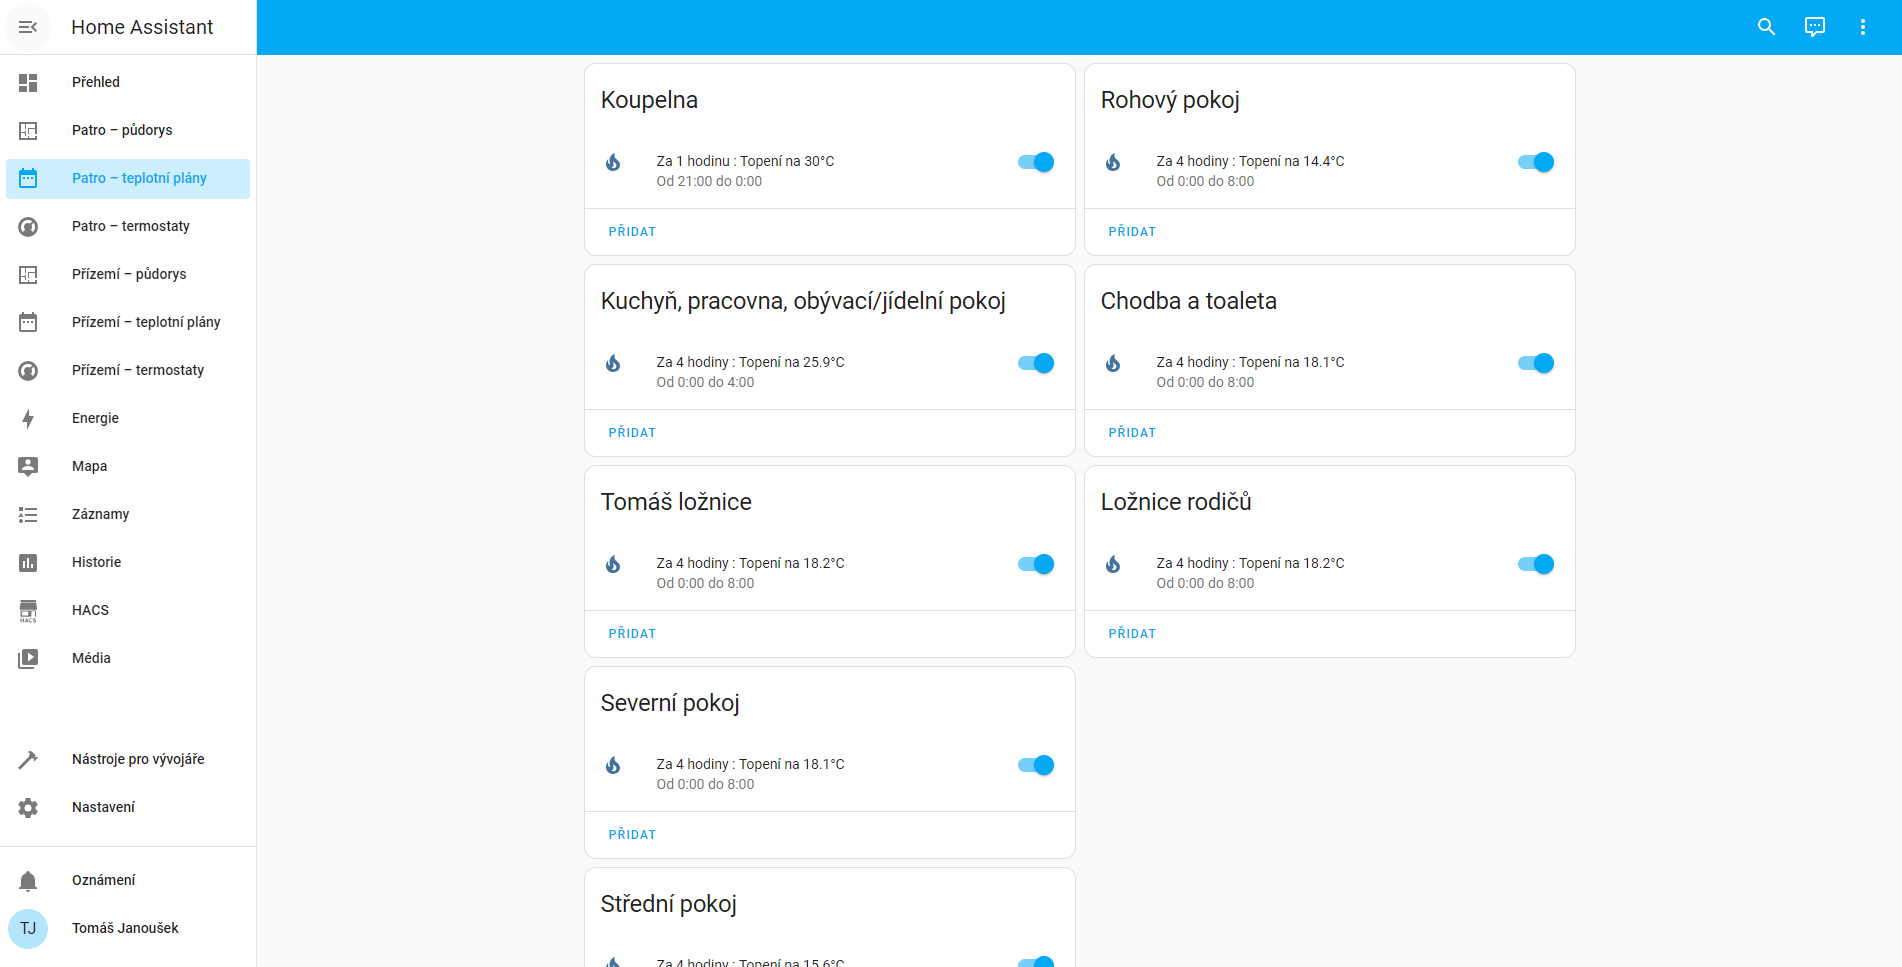
\includegraphics[width=1\textwidth]{pictures/czech/software/temperature-plan-ground-floor.png}
    \caption{Teplotní plány pro přízení.}
    \label{fig:temperature-plan-ground-floor}
\end{figure}
\end{Czech}

\begin{Czech}
Pro každou místnost je předdefinovaný teplotní plán. Pro úpravu stačí na něho kliknout, zobrazí se obrázek \ref{fig:temperature-plan-thermostat}. Pro úpravu teploty daného úseku stačí kliknout na vybraný úsek a pomocí posuvníku dole změnit teplotu. Případně je možné daný úsek přidat nebo smazat. Následně dané nastavení uložit tlačítek vpravo dole. Na základě takto nastaveného teplotního plánu dochází k nastavení požadované teplotu to nástěnného snímače podle kterého se řídí  vytápění dané místnosti.
\end{Czech}

\begin{Czech}
\begin{figure}[H]
    \centering
    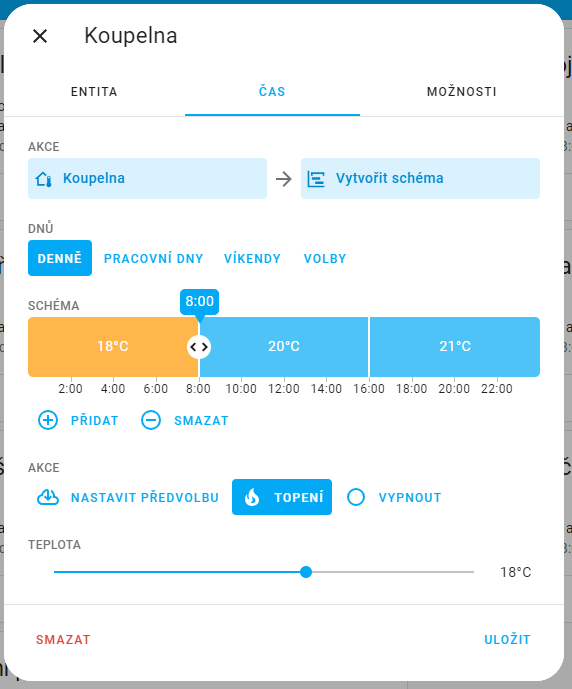
\includegraphics[width=0.5\textwidth]{pictures/czech/software/temperature-plan-thermostat.png}
    \caption{Nastavení/úprava teplotního plánu.}
    \label{fig:temperature-plan-thermostat}
\end{figure}
\end{Czech}

% ========================================

\begin{Czech}
\subsubsection{Módy řízení}
\end{Czech}
\label{sec:control-modes}

\begin{Czech}
Na základě zvoleného módu řízení (obrázek \ref{fig:control-modes}) dojde k řízení topné spirály v zásobníku otopné vody. Meze min. horní čidlo a max. střední čidlo se berou podle vybrané letního nebo zimního módu, obrázek \ref{fig:switching-heating-coil}. Diagram řízení pro daný mód je na obrázku \ref{fig:diagram-control-modes}.
\end{Czech}

\begin{Czech}
\begin{figure}[H]
    \centering
    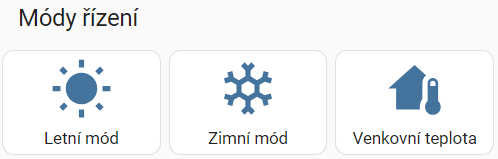
\includegraphics[width=0.7\textwidth]{pictures/czech/software/control-modes.png}
    \caption{Módy řízení.}
    \label{fig:control-modes}
\end{figure}
\end{Czech}

\begin{Czech}
\begin{figure}[H]
    \centering
    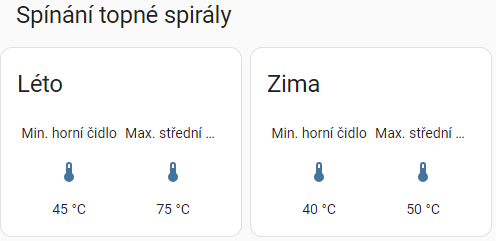
\includegraphics[width=0.7\textwidth]{pictures/czech/software/switching-heating-coil.png}
    \caption{Spínání topné spirály.}
    \label{fig:switching-heating-coil}
\end{figure}
\end{Czech}

\begin{Czech}
\begin{figure}[H]
    \centering
    \def\svgwidth{1\columnwidth}
    \graphicspath{{pictures/czech/software/svg/}}
    \input{pictures/czech/software/svg/diagram-control-modes.pdf_tex}
    \caption{Diagram módu řízení.}
    \label{fig:diagram-control-modes}
\end{figure}
\end{Czech}

% ========================================

\begin{Czech}
\subsubsubsection{Ostatní nastavení}
\end{Czech}

\begin{Czech}
V části ostatní nastavení je možné nastavit hysterezi spirály využívanou v \textbf{módech řízení}. V „\textit{Min. venkovní teplota pro letní mód}“ se definuje mez pro určení, zda se jedná o letní nebo zimní mód. Pokud je venkovní teplota vetší nebo rovna této mezi zvolí se letní mód jinak zimní.
\end{Czech}

\begin{Czech}
\begin{figure}[H]
    \centering
    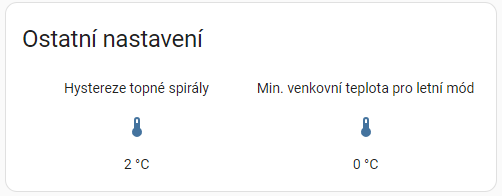
\includegraphics[width=0.7\textwidth]{pictures/czech/software/other-settings.png}
    \caption{Ostatní nastavení.}
    \label{fig:other-settings}
\end{figure}
\end{Czech}

% ========================================

\begin{Czech}
\subsubsection{Krby – spínání čerpadel}
\end{Czech}

\begin{Czech}
Na obrázku \ref{fig:diagram-fireplace} je diagram pro sepnutí oběhových čerpadel pro krby v případě zatopení. Pro všechny krbová čerpadla je toto nastavení stejné, liší se pouze min. mez pro sepnutí podle obrázku \ref{fig:fireplace-switching-pumps}.
\end{Czech}

\begin{Czech}
\begin{figure}[H]
    \centering
    \def\svgwidth{1\columnwidth}
    \graphicspath{{pictures/czech/software/svg/}}
    \input{pictures/czech/software/svg/diagram-fireplace.pdf_tex}
    \caption[]{Diagram spínání oběhových čerpadel pro krby.}
    \label{fig:diagram-fireplace}
\end{figure}
\end{Czech}

\begin{Czech}
\begin{figure}[H]
    \centering
    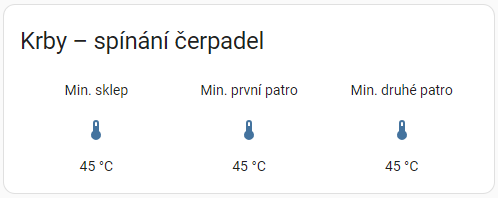
\includegraphics[width=0.7\textwidth]{pictures/czech/software/fireplace-switching-pumps.png}
    \caption{Nastavení min. mezí pro sepnutí oběhových čerpadel pro krby v případě zatopení.}
    \label{fig:fireplace-switching-pumps}
\end{figure}
\end{Czech}

\begin{Czech}
\tipbox{Poznámka}{Toto nastavení je zcela nezávislé na dalších nastavení systému. \mbox{V případě} zatopení musí dojít vždy \mbox{k sepnutí} čerpadla.}
\end{Czech}

% ========================================

\begin{Czech}
\subsubsection{LED indikace – mezí parametry zásobníku teplé vody}
\end{Czech}
\label{sec:led-indication}

\begin{Czech}
Na obrázku \ref{fig:led-indication} jsou nastavitelné meze pro ovládání signalizačních LED pro zásobník otopné vody. Jednotlivé LED označují natopení respektive chladnou část zásobníku otopné vody. Červená LED je pro spodní část, oranžová LED pro střední část a modrá LED pro horní část zásobníku otopné vody. V případě, že teplota ve spodní respektive střední části je větší než meze nastavené pro červenou respektive oranžovou LED, dojde k rozsvícení červené respektive oranžové LED. V případě, že teplota v horní části je nižší než mez pro modrou LED, dojde k rozsvícení modré LED. Diagram pro červenou respektive oranžovou LED je na obrázku \ref{fig:diagram-red-orange-led-indication}. Diagram pro modrou LED je na obrázku \ref{fig:diagram-blue-led-indication}.
\end{Czech}

\begin{Czech}
\begin{figure}[H]
    \centering
    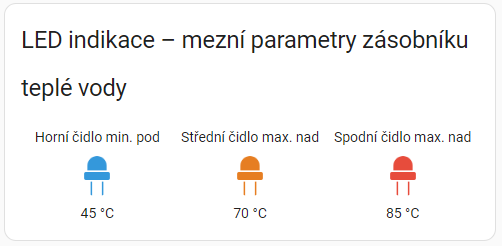
\includegraphics[width=0.65\textwidth]{pictures/czech/software/led-indication.png}
    \caption{Meze pro ovládání signalizační LED pro zásobník otopné vody.}
    \label{fig:led-indication}
\end{figure}
\end{Czech}

\begin{Czech}
\begin{figure}[H]
    \centering
    \def\svgwidth{1\columnwidth}
    \graphicspath{{pictures/czech/software/svg/}}
    \input{pictures/czech/software/svg/diagram-red-orange-led-indication.pdf_tex}
    \caption{Diagram ovládání červené a oranžové signalizační LED.}
    \label{fig:diagram-red-orange-led-indication}
\end{figure}
\end{Czech}

\begin{Czech}
\begin{figure}[H]
    \centering
    \def\svgwidth{1\columnwidth}
    \graphicspath{{pictures/czech/software/svg/}}
    \input{pictures/czech/software/svg/diagram-blue-led-indication.pdf_tex}
    \caption{Diagram ovládání modré signalizační LED.}
    \label{fig:diagram-blue-led-indication}
\end{figure}
\end{Czech}

\begin{Czech}
\tipbox{Poznámka}{Toto nastavení je zcela nezávislé na dalších nastavení systému.}
\end{Czech}

% ====================  STOP Tab settings ====================

% ====================  START Tab devices ====================
\begin{Czech}
\subsection{Záložka zařízení}
\end{Czech}

\begin{Czech}
\subsubsection{Koncová zařízení}
\end{Czech}

\begin{Czech}
V záložce \textbf{zařízení} obrázek \ref{fig:tab-devices} (horní modré menu) jsou vidět v části „\textit{Koncová zařízení}“ stav respektive možnost zapnout/vypnout dané zařízení, obrázek \ref{fig:end-devices}. V případě, že uživatel chce měnit stav zařízení musí uvést tlačítko „\textit{Manuální ovládání zařízení}“ do stavu zapnuto (modrý stav tlačítka), pak je možné manuálně ovládat zřízení. \mbox{V případě}, že uživatel změní stav zařízení bez možnosti „\textit{Manuální ovládání zařízení}“ může dojít k přepsaní uživatelského nastavení zařízení podle stavu ze systému. U LED je možné pouze vidět stav zapnuto/vypnuto manuální ovládání LED není k dipozici.
\end{Czech}

\begin{Czech}
\begin{figure}[H]
    \centering
    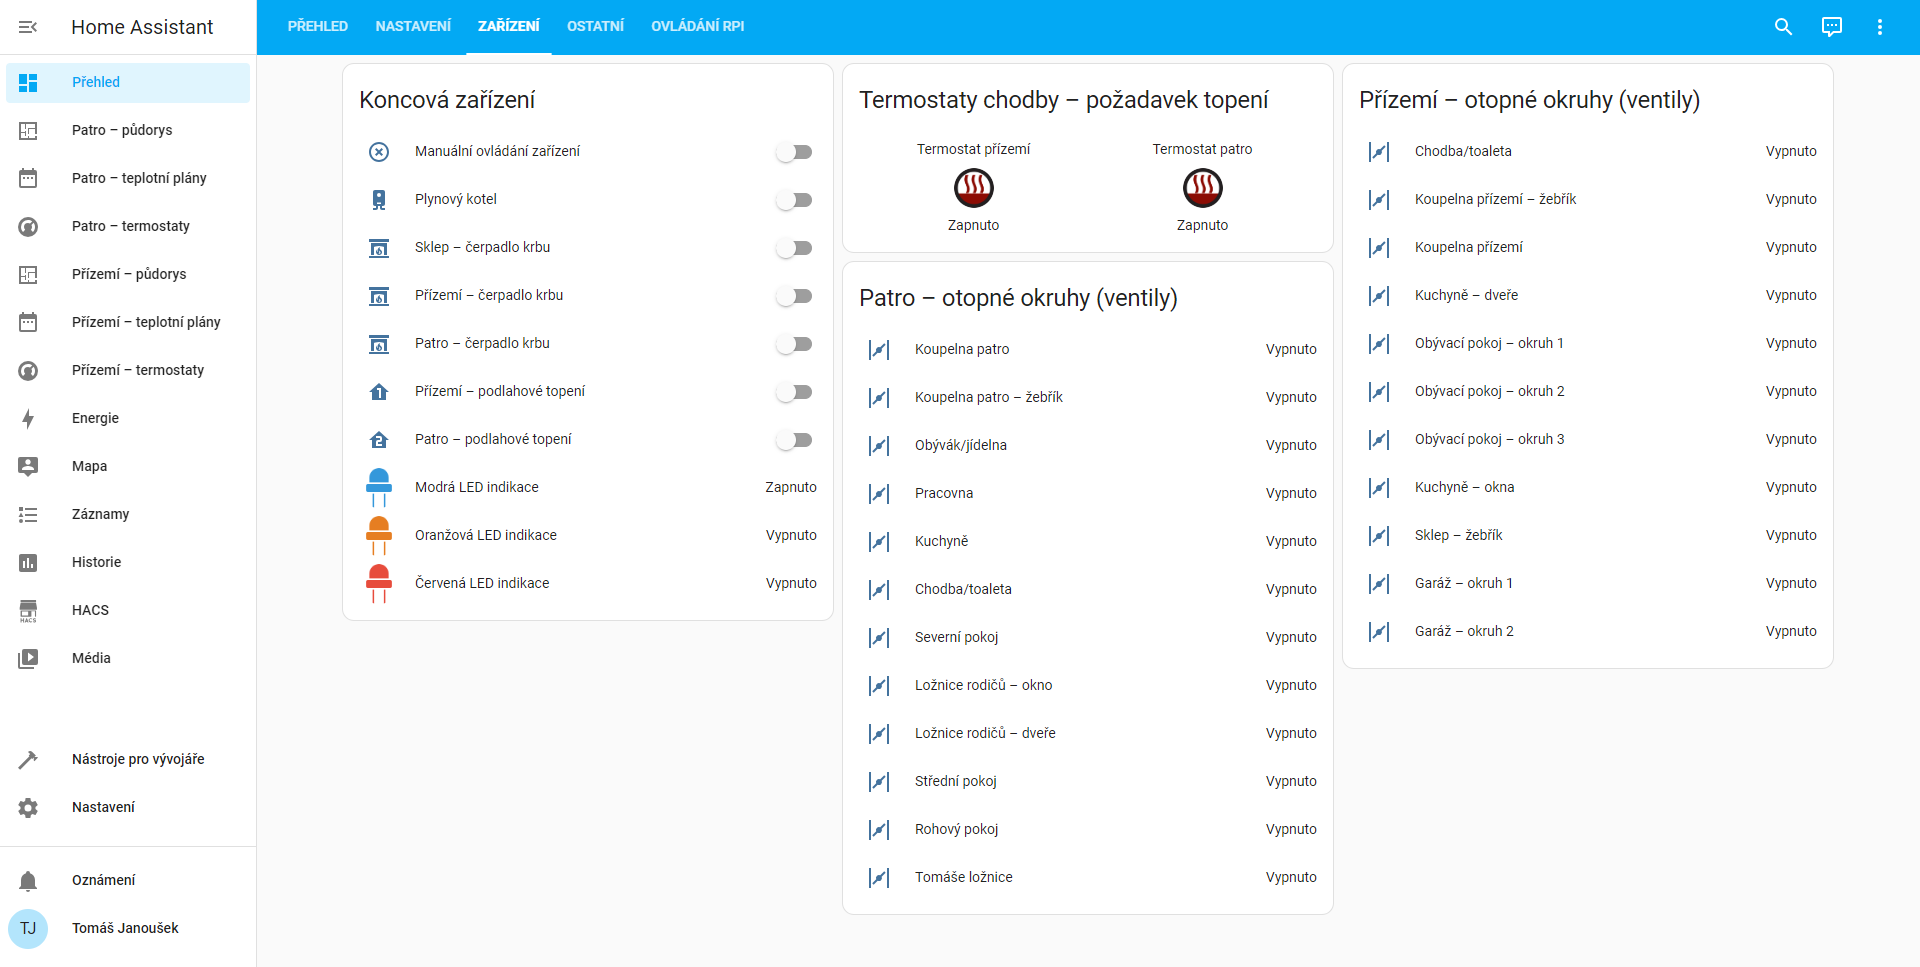
\includegraphics[width=1\textwidth]{pictures/czech/software/tab-devices.png}
    \caption{Záložka zařízení.}
    \label{fig:tab-devices}
\end{figure}
\end{Czech}

\begin{Czech}
\begin{figure}[H]
    \centering
    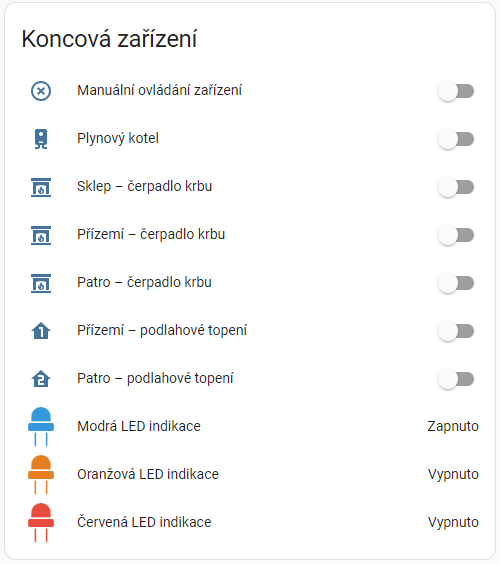
\includegraphics[width=0.6\textwidth]{pictures/czech/software/end-devices.png}
    \caption{Koncová zařízení.}
    \label{fig:end-devices}
\end{figure}
\end{Czech}

\begin{Czech}
\tipbox{Pozor!!!}{Pokud uživatel nastaví tlačítko „Manuální ovládání zařízení“ do stavu zapnuto. Systém \textbf{nemůže} následně zařízení ovládat podle nastavené automatizace. Je nutné vždy tlačítko vrátit do stavu \textbf{vypnuto}. }
\end{Czech}

% ========================================

\begin{Czech}
\subsubsection{Termostaty chodby – požadavek topení}
\end{Czech}

\begin{Czech}
Na obrázku \ref{fig:corridor-thermostats2} je vidět stav zapnuto/vypnuto pro chodbové termostaty. Toto nastavení se dále používá v módu vytápění „Řízení teploty z chodbových termostatů“, více informací v sekci „Řízení teploty z chodbových termostatů“.
\end{Czech}

\begin{Czech}
\begin{figure}[H]
    \centering
    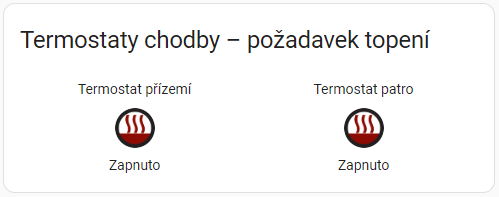
\includegraphics[width=0.6\textwidth]{pictures/czech/software/corridor-thermostats.png}
    \caption{Termostaty chodby – požadavek topení.}
    \label{fig:corridor-thermostats2}
\end{figure}
\end{Czech}

% ========================================

\begin{Czech}
\subsubsection{Přízemí/patro – otopné okruhy (ventily)}
\end{Czech}

\begin{Czech}
Na obrázku \ref{fig:heating-circuits-ground-floor2} je vidět stav zapnuto/vypnuto ventilu pro jednotlivé otopné okruhy, rozdělené do přízemí a patra. Pokud uživatel manuálně zapne ventil přes vypínač na zónovém regulátoru umístěný na rozdělovačích podlahové vytápění. Stav zapnutí se nepromítne do systému, stav zapnuto není v systému vidět. Manuální zapnutí přes vypínač používat jen v případě, že systém je nefunkční. Při takto manuálním zapnutí ventilu respektive otopného okruhu dojde k sepnutí příslušného oběhového čerpadla. Uživatel nemá možnost manuálně přes systém zapínat jednotlivé otopné okruhy, pouze vidět jejich stav. Další informace o ovládání otopných okruhů je v části \ref{sec:temperature-control} „\textit{Řízení teploty}“.
\end{Czech}

\begin{Czech}
\begin{figure}[H]
    \centering
    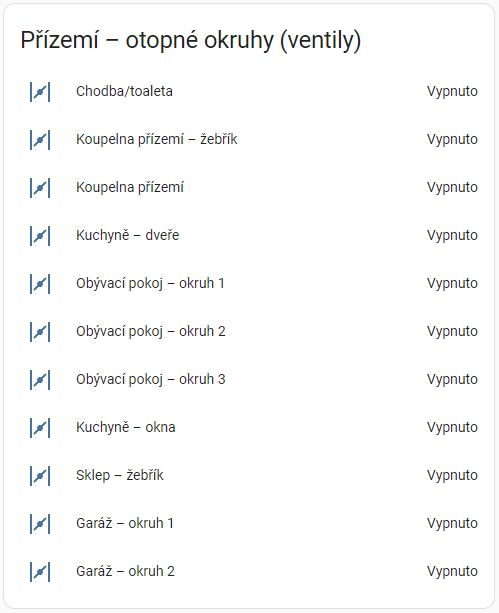
\includegraphics[width=0.6\textwidth]{pictures/czech/software/heating-circuits-ground-floor.png}
    \caption{Přízemí – otopné okruhy (ventily).}
    \label{fig:heating-circuits-ground-floor2}
\end{figure}
\end{Czech}

% ========================================

\newpage
\begin{Czech}
\subsection{Záložka ostatní}
\end{Czech}

\begin{Czech}
V záložce \textbf{ostatní} obrázek \ref{fig:tab-others} (horní modré menu) je vidět nastavení pro „\textit{Ovládaní čerpadel – vodní kámen}“. Toto je nastavení je užitečné pro pravidelné „protočení“ krbových oběhový čerpadel v definovaný den a hodině s délkou spuštění. Pokud čerpadla delší dobu stojí, může dojít k zatuhnutí vlivem vodního kamene, toto nastavení tento jev minimalizuje. 
\end{Czech}

\begin{Czech}
\begin{figure}[H]
    \centering
    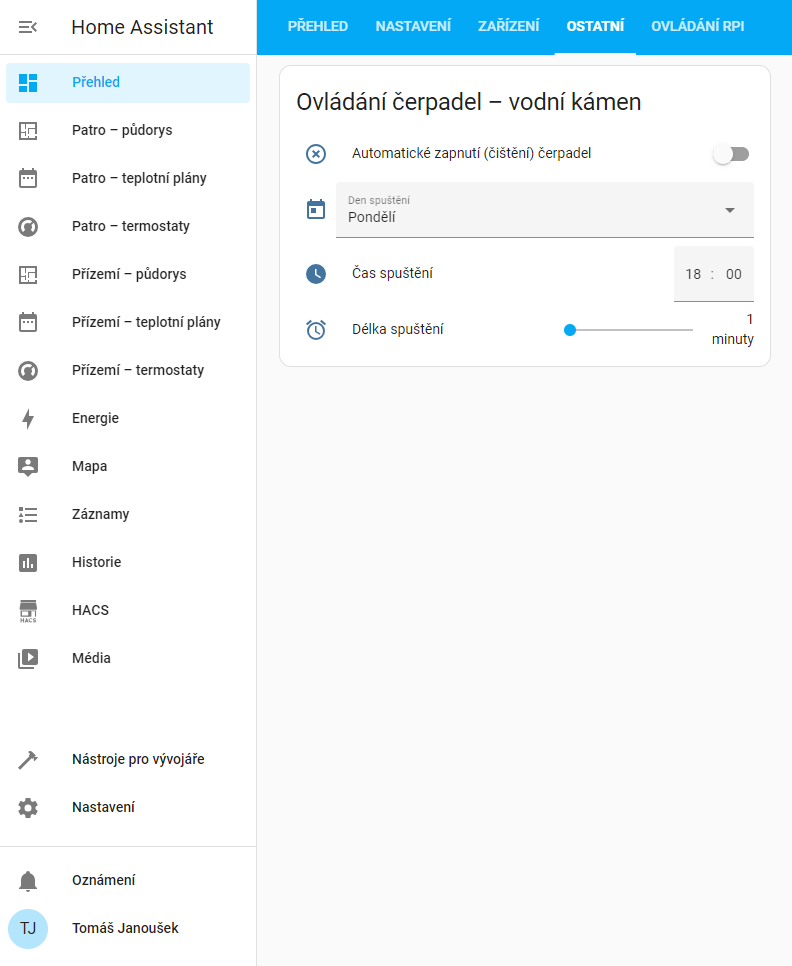
\includegraphics[width=0.6\textwidth]{pictures/czech/software/tab-others.png}
    \caption{Záložka ostatní.}
    \label{fig:tab-others}
\end{figure}
\end{Czech}

% ========================================

\newpage
\begin{Czech}
\subsection{Přízemí/patro – půdorys}
\end{Czech}

\begin{Czech}
V záložce \textbf{Přízemí/patro – půdorys} obrázek \ref{fig:floor-plan-first-floor} (levé menu) je vidět půdorys pro přízemí/patro domu s jednotlivými aktuálně naměřenými teplotami, požadovanými teplotami, stavem topení v dané místnosti a stavem čerpadel respektive stavem topením v krbu. Po kliknutí na danou teplotu je možné měnit požadovanou teplotu apod. toto nastavení se propisuje do jednotlivých termostatů v místnosti.
\end{Czech}

\begin{Czech}
\begin{figure}[H]
    \centering
    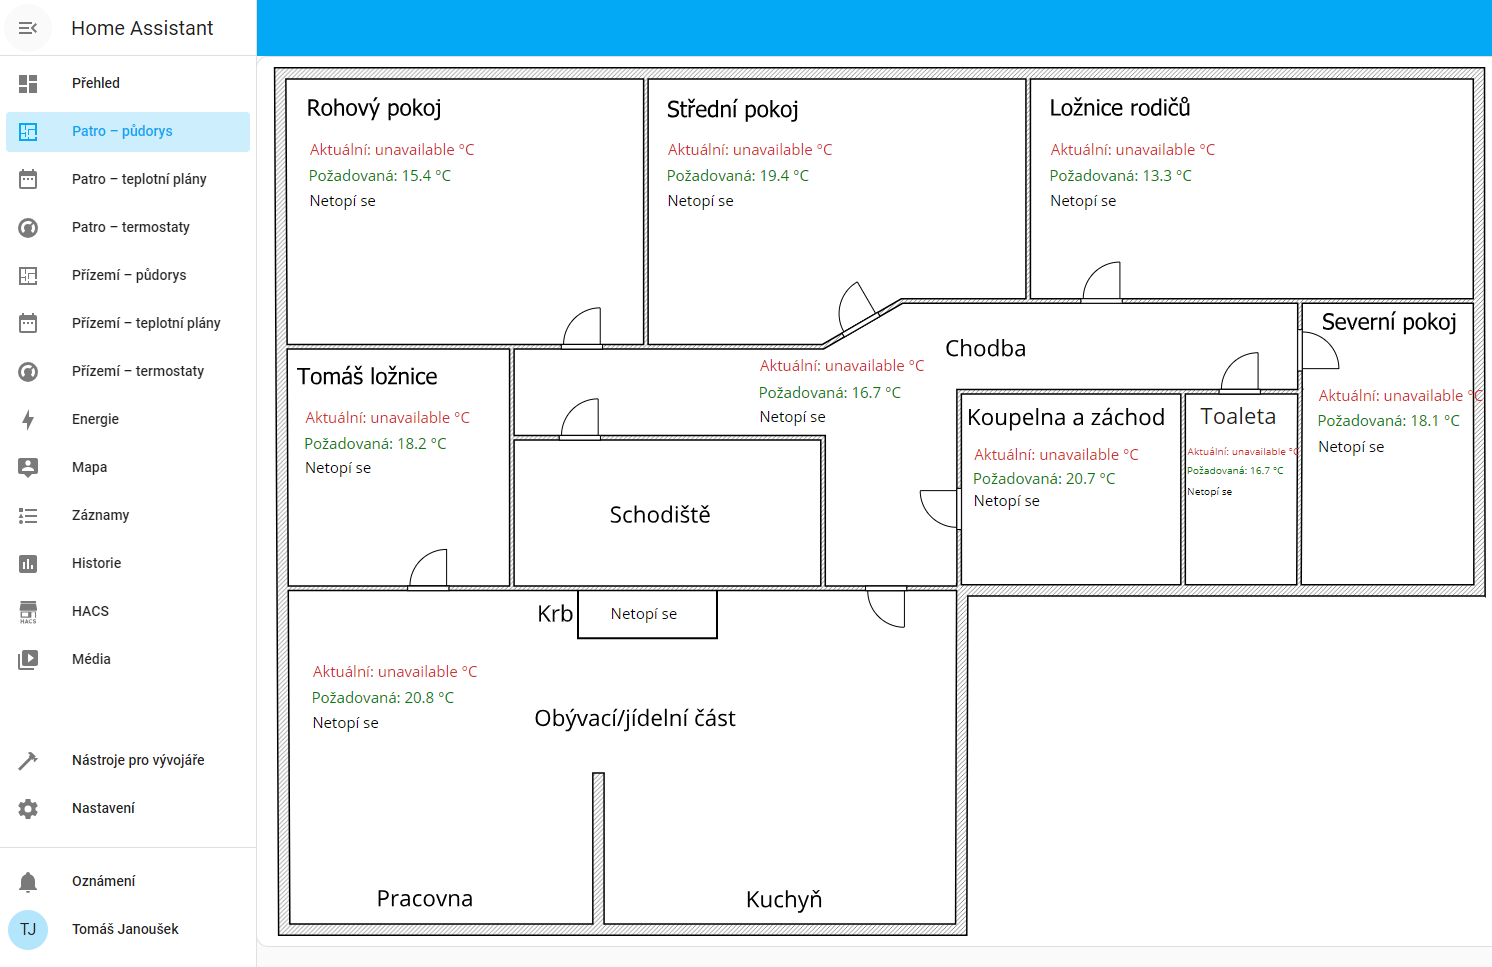
\includegraphics[width=1\textwidth]{pictures/czech/software/floor-plan-first-floor.png}
    \caption{Patro – půdorys.}
    \label{fig:floor-plan-first-floor}
\end{figure}
\end{Czech}
